\chapter{Implementierung}\label{Chap:Implementierung}

\section{Projektplan für den Feasibility Check}
Einbauen des GANT-Diagramms / Projektplans


\begin{figure}[!h]
    \centering
    \includegraphics[width=1\textwidth]{bilder/Roadmap.pdf}
    \caption{Feasibility Check Roadmap}
    \label{fig:roadmap}
\end{figure}
\section{Entwicklungsumgebung}
Tools und Technologien, die verwendet wurden (IDE, Frameworks, Datenbank-Tools).
Angular, Visual Studio Code, 
C\#, Visual Studio,
Oracle, Pl sql developer

\section{Implementierung des Feasibility Checks}
Detaillierte Beschreibung des Implementierungsprozesses.
\section{Integration}
Wie die verschiedenen Teile (Frontend, Backend, Datenbank) miteinander interagieren.

\begin{figure}[!h]
    \centering
    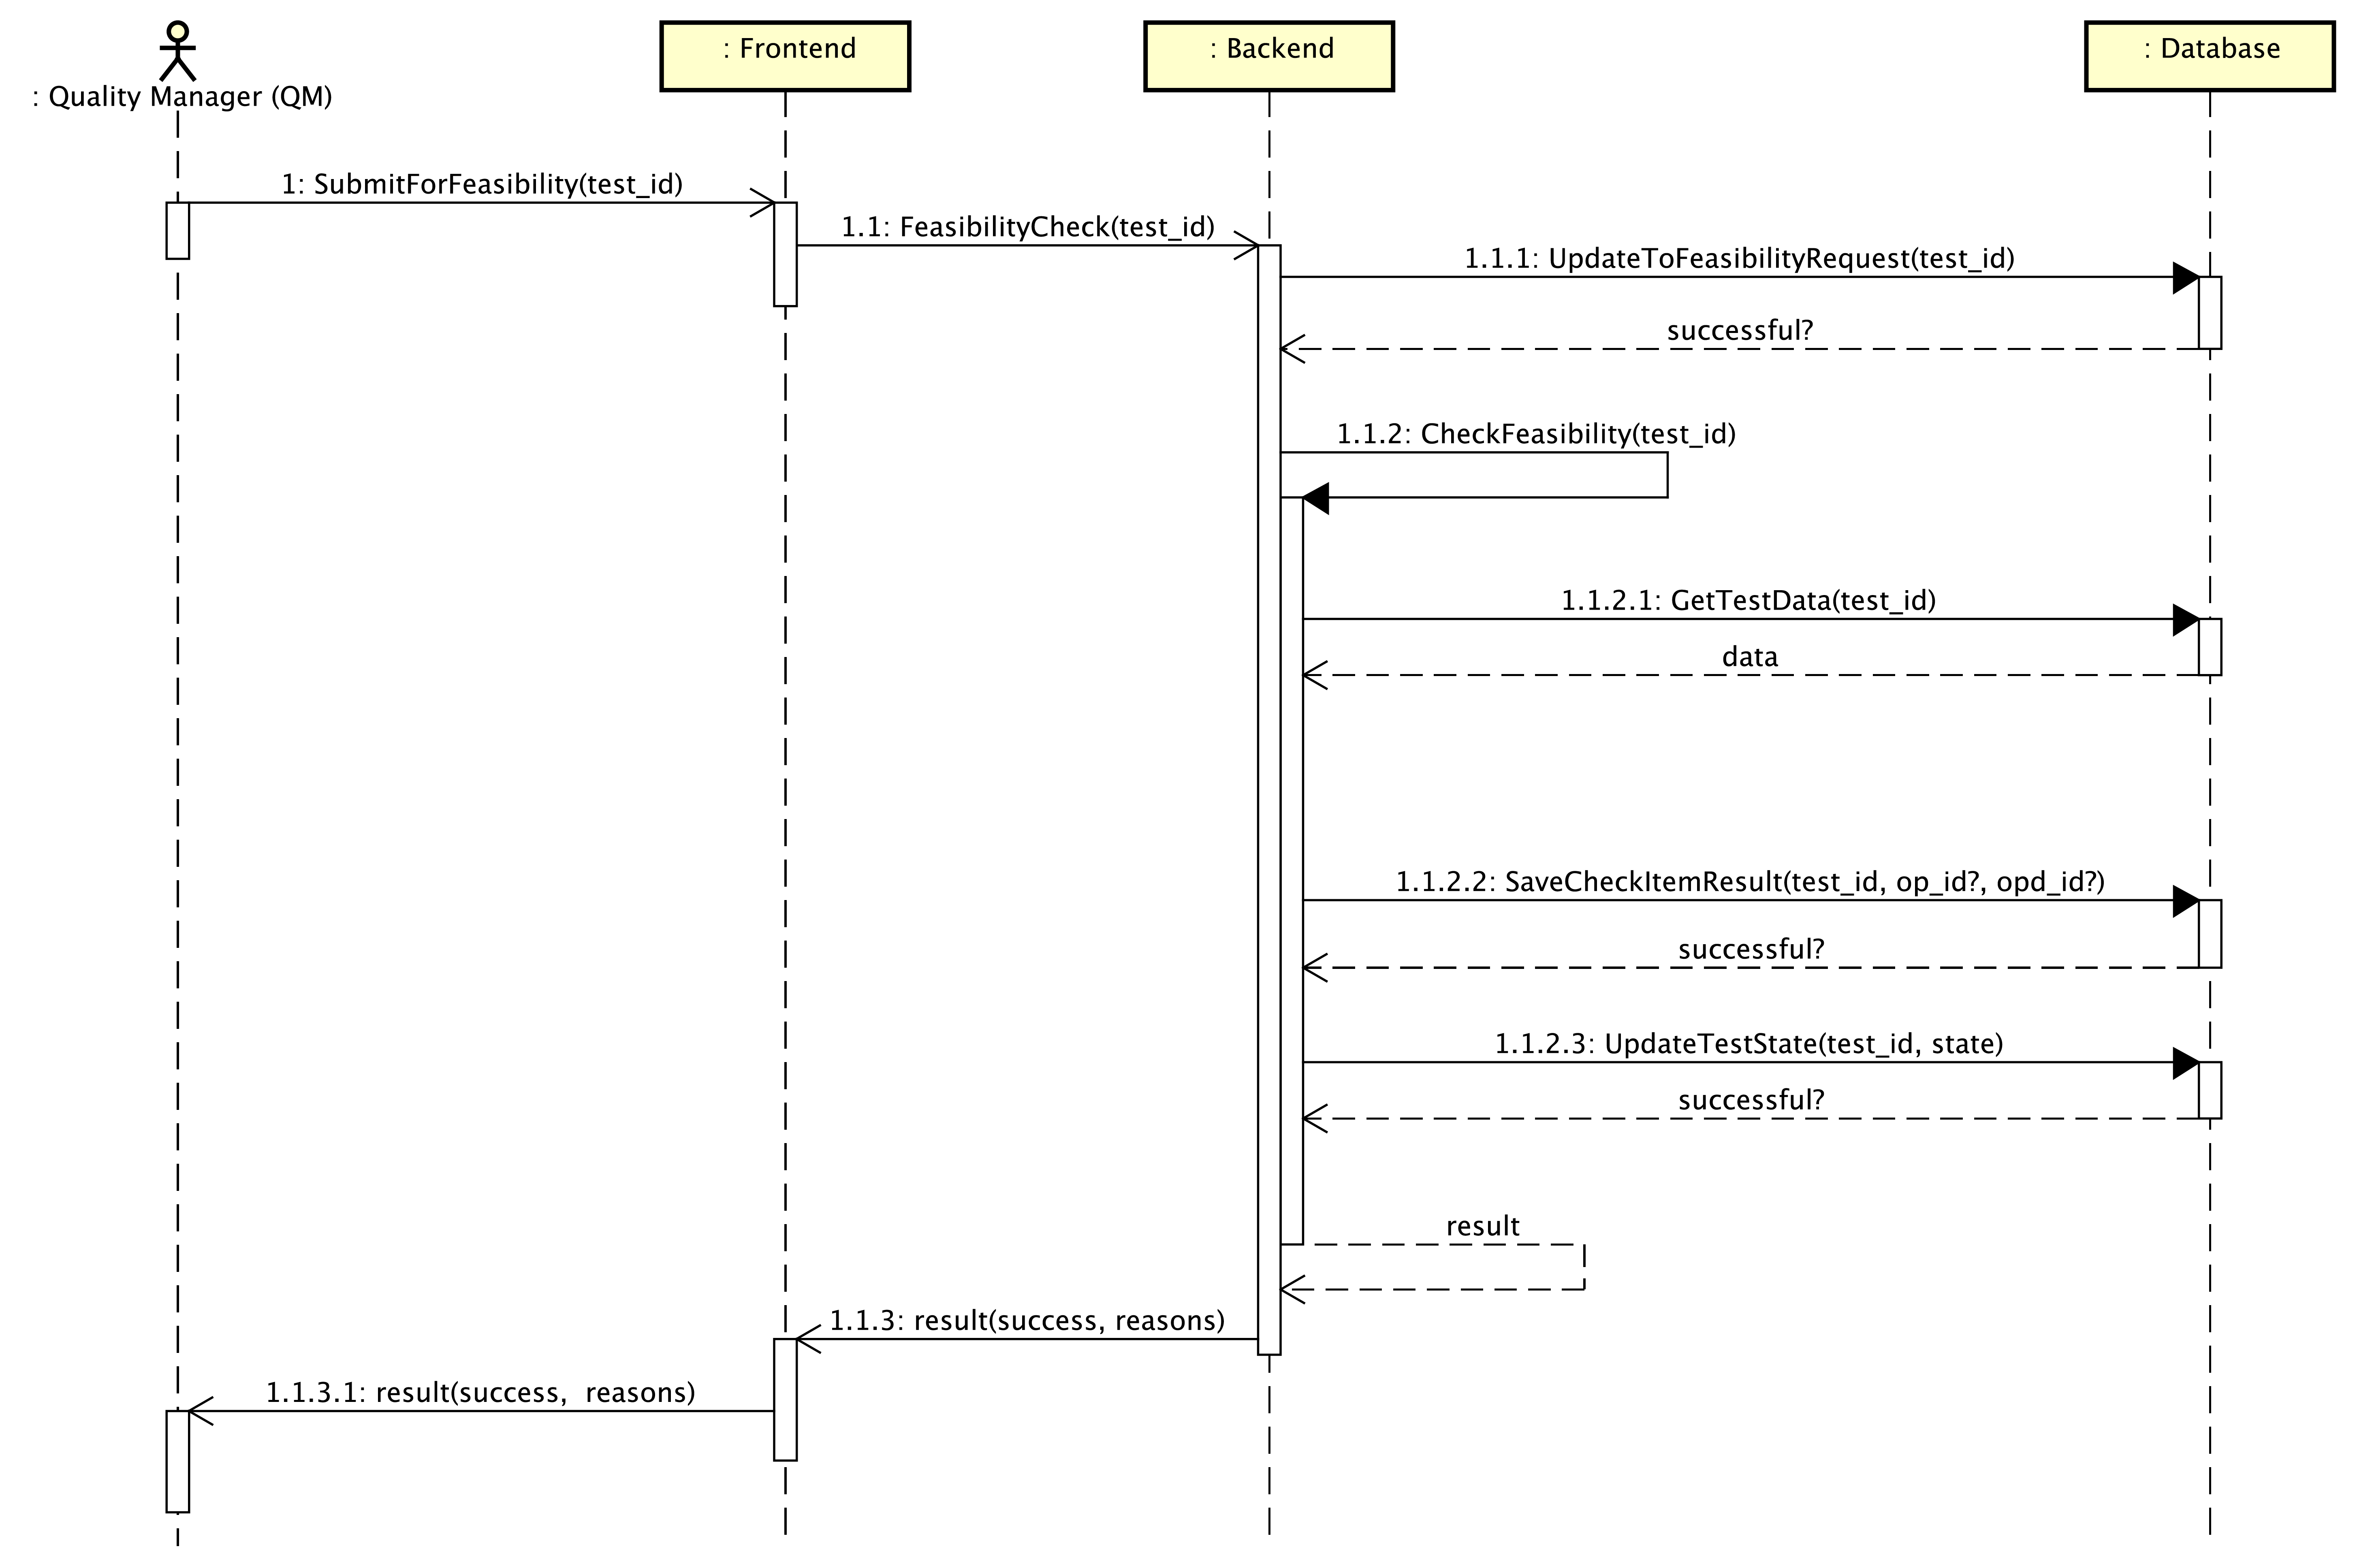
\includegraphics[width=1\textwidth]{bilder/Sequence-Integration.png}
    \caption{Sequenz-Diagramm FeasibilityCheck}
    \label{fig:sequence-diagram}
\end{figure}